\documentclass[10pt,A4paper]{article}

\usepackage{acronym}
\usepackage{amsmath,amssymb}
\usepackage[aboveskip=1pt,labelfont=bf,labelsep=period,justification=raggedright,singlelinecheck=off]{caption}
\usepackage{changepage}
\usepackage{cite}
\usepackage{nameref,hyperref}
\usepackage[right]{lineno}
\usepackage[nopatch=eqnum]{microtype}

\usepackage{xcolor}

\usepackage[outputdir=out]{minted}
\definecolor{bg}{HTML}{282828} % fro https://github.com/kevinsawicki/monokai
\setminted{autogobble=true,bgcolor=bg,linenos=true,style=monokai}

\bibliographystyle{abbrv}

% Header and Footer with logo
\usepackage{lastpage,fancyhdr,graphicx}
\usepackage{epstopdf}
\pagestyle{fancy}
\fancyhf{}
\rfoot{\thepage/\pageref{LastPage}}
\renewcommand{\headrulewidth}{0pt}
\renewcommand{\footrule}{\hrule height 2pt \vspace{2mm}}
\lfoot{\today}

\newcommand{\etal}{{\textit{et al.}}}
\newcommand{\mbx}{\mathbf{x}}
\newcommand{\mbu}{\mathbf{u}}
\newcommand{\mbp}{\mathbf{p}}
\newcommand{\mby}{\mathbf{y}}
\providecommand{\keywords}[1]{\textbf{Keywords } #1}


% Create acronyms to use in text
\newacro{ode}[ODE]{Ordinary Differential Equation}
\newacro{oed}[OED]{optimal experimental design}
\newacro{fim}[FIM]{Fisher information matrix}


\begin{document}
% ########################################################################
% ########################################################################
\vspace*{0.2in}
% Title must be 250 characters or less.
\begin{flushleft}
{\Large
\textbf\newline{Model Calibration with Process Variables depending on Environmental Parameters}}
\newline
\\
Polina Gaindrik\textsuperscript{1,2,3},
Jonas Pleyer\textsuperscript{1,2},
Christian Fleck\textsuperscript{1,2,3}
\\
\bigskip
\textbf{1} \href{https://www.fdm.uni-freiburg.de/spatsysbio}{University of Freiburg}\\
\textbf{2} \href{https://www.fdm.uni-freiburg.de/spatsysbio}{Freiburg Center for Data Analysis and Modeling}\\
\textbf{3} \href{https://tsenso.com/en/}{Tsenso}\\
\bigskip

\end{flushleft}
% ########################################################################
% ########################################################################
\section*{Abstract}
\linenumbers
Parameter estimation is a significant part of the model building that is always accompanied by uncertainty.
Experimental design allows optimization of the observation conditions and reduces the uncertainty of the parameter estimation as well as the number of measurements required for meaningful model quantification.
In this chapter, we provide instructions for finding the optimal experimental design using the Baranyi and Roberts growth model with the 'square root' secondary model for the maximum growth rate as a specific example from Predictive Microbiology. 
The guidelines are supposed to clarify the procedure and make it more accessible for the reader familiar with the field of Systems Biology.
We provide Python-written software for the \acp{ode}-based models that optimize the measurement times and inputs of the model.


\keywords{Optimal experimental design, Parameter estimation, Fisher Information matrix, Identifiability, Uncertainty}

%
%
%
% ########################################################################
% ########################################################################
\section*{Introduction}
% \begin{figure}[h]
% 	\inputminted[linenos,firstline=57,lastline=79]{python}{../model-design-fischer-information-matrix/pool_model.py}
% 	\caption{Sample code written in Python~\cite{rossumPythonLanguageReference2010}.}
% \end{figure}
%
\begin{enumerate}
	\item Why do we want parameter estimation and experimental design?
	\item Flow-Chart Experimental Design
	\item Citations to common methods
\end{enumerate}


Mathematical modeling is a widely used tool to describe, understand and predict further behavior of living systems.
In particular, in the field of Predictive Biology, one can find a large variety of works that dwell on building models of different levels of complexity controlled by model parameters, e.g., to describe bacteria growthBased on a chosen model structure, these parameters can be estimated from the gathered experimental data.
Taking into account that the real experimental data always contains measurement noise, the parameter estimates can be only provided with some uncertainty. 
To decrease the error of the parameter values, not only enough experimental data should be gathered but the quality of this data is also pretty sufficient.
That rises quite an important question of finding the \ac{oed} where optimized experimental conditions and/or times allow one to reduce the number of measurements without loss of information thus sparing an effort of experimenters \cite{derlindenImpactExperimentDesign2013, balsa-cantoe.bangaj.r.COMPUTINGOPTIMALDYNAMIC2008}. 
In general, \ac{oed} can be used not only for the parameter estimation of the model but also for model discrimination to choose between different model structures \cite{kreutzSystemsBiology2009, stamatiOptimalExperimentalDesign2016}.
However, in this chapter, we would like to cover more deeply the methods for improving the parameter estimation of the model.
According to this, using tools of Statistics and specifically the Fisher information, several criteria were developed to assess data quality. 
The review of these different possible criteria the reader can find for example in works \cite{atkinsonDevelopmentsDesignExperiments1982, franceschiniModelbasedDesignExperiments2008}.
Depending on the goal, a researcher faces an important choice which among these sometimes contradicting each other criteria is the most suitable one for a particular case.
On the other hand, using the multi-objective approach, some attempts were made to improve the experimental design by combining these criteria \cite{telenOptimalExperimentDesign2012, logistRobustMultiobjectiveOptimal2011}.
If we are talking about predictive microbiology, one of the promising applications of the \ac{oed} is to optimize the temperature profile with the time of the experiment as it was done by García \etal \cite{garciaQualityShelflifePrediction2015} and Versyck \etal \cite{versyckIntroducingOptimal1999}.
Or, for example, Balsa-Canto \etal compared equidistant and optimized measurement times for such bacteria growth models as Baranyi and Roberts model and Bigelow model and have shown improvement in the latter case \cite{balsa-cantoe.bangaj.r.COMPUTINGOPTIMALDYNAMIC2008}.

\begin{figure}[H]
    \centering
    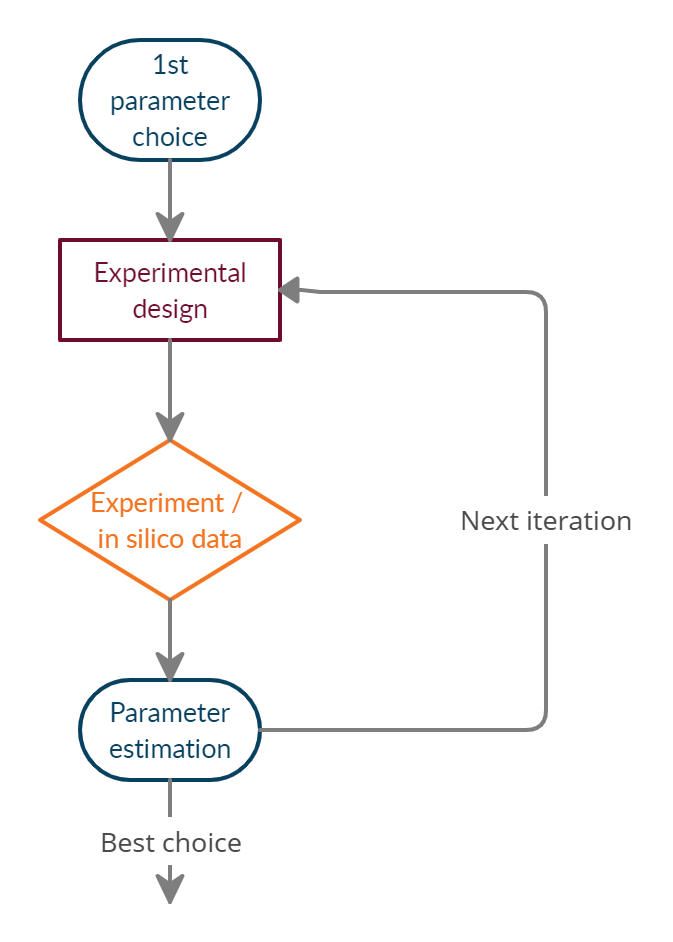
\includegraphics[scale=0.3]{Figures/scheme.png}
    \caption{The iterative process of model optimization for parameter estimation.}
    \label{fig:expdesign_scheme}
\end{figure}
In the beginning, we would like to briefly describe the whole iterative process of model building (see Fig. \ref{fig:expdesign_scheme}).
First of all, based on the literature review or some prior data from pilot experiments the first parameter estimation of the chosen model structure should be done.
The obtained values can be applied to propose the first optimal experimental design accounting for different constraints, e.g., the lab limitations, human resources, etc. 
Depending on availability, either real or numerical experiment should be conducted based on this design to gather measurement or in-silico data. 
This new data can be used for the new parameter estimations values with corresponding uncertainties.
After this, using new parameter values, the process can be repeated several times to increase the precision of the parameter estimates till the desired accuracy is achieved.







%
%
%
% ########################################################################
% ########################################################################
\section*{Materials and Methods}
This tutorial expects a working installation of the popular scripting language Python $\geq3.7$~\cite{rossumPythonLanguageReference2010}.
For installation instructions, please refer to the website \href{https://www.python.org/downloads/}{python.org}.
We have developed \mintinline[bgcolor=white,style=emacs]{bash}{FisInMa}, which is a set of tools to calculate the Sensitivity and Fischer Information Matrix and do parameter space exploration in order to find optimal results.
Users can obtain it by installing \mintinline[bgcolor=white,style=emacs]{bash}{FisInMa} from \href{https://pypi.org/project/FisInMa/0.0.1/}{pypi.org}.
The python website has guides for installing packages \href{https://packaging.python.org/en/latest/tutorials/installing-packages/}{packaging.python.org/}.
Most Unix-Based systems (eg. GNU/Linux) and Mac-OS can use \mintinline[bgcolor=white,style=emacs]{bash}{pip}
\begin{minted}[bgcolor=white]{bash}
pip install FisInMa
\end{minted}
or \mintinline[bgcolor=white,style=emacs]{bash}{conda} to install the desired package.
\begin{minted}[bgcolor=white]{bash}
conda install FisInMa
\end{minted}
%
%
% ########################################################################
\subsection*{Model Formulation}
\subsubsection*{Theory}
\begin{enumerate}
    \item Define ODE, Jacobian
    \item Which parameters are present?
    \item Differnce between Q-Values, P-Values, Const
\end{enumerate}

The first important step a reader should do to conduct their Experimental Design is to define a model structure.
In this chapter, we restrict ourselves to a quite popular case in Predictive Microbiology and assume that biological system is described by a system of \acp{ode}
\begin{equation}
    \begin{cases}
    \dot \mbx (t) = f(\mbx, t, \mbu, \mbp, c) \\
    \mbx (0) = \mbx_0
    \label{eq:ode_general}
    \end{cases}.
\end{equation}
Here $\mbx = (x_1, x_2, ..., x_n)$ is a vector of state variables of the system with initial condition $\mbx_0$, $t$ is time, $\mbu$ is a vector of an externally controlled inputs, $\mbp$ are the parameters of the system and $c$ are the constants.
Here, it is important to differentiate between constants and parameters.
The main difference is that we assume constant values to be known for sure, so they shouldn't be estimated from experimental data.
On the other hand, parameters are the quantities of interest and their estimation is our goal, Experimental Design should be chosen relying on them.
Another important choice to be done is to define the observables of the system $\mby$, which quantities and at which times $t_i$ should be measured.
\begin{equation}
    \mby (t_i) = g(\mbx (t_i), t, \mbu, \mbp, c) + \epsilon (t_i),
    \label{eq:observ_general}
\end{equation}
where the function $g$ describes the model output and $\epsilon$ is the measurement noise. 
The observational noise is often assumed to be an independently distributed Gaussian noise.

Here, to demonstrate how Experimental Design works, we will refer to a widely used Baranyi and Roberts model (1994) that can be used, for example, to describe bacteria growth.
The model is introduced by two state variables $\mbx = (x_1, x_2)$, where $x_1(t)$ denotes the cell concentration of a bacterial population at the time $t$ and $x_2(t)$ defines a physiological state of the cells, the process of adjustment (lag-phase):
\begin{equation}
    \begin{cases}
    \dot x_1(t) = \frac{x_2(t)}{x_2(t) + 1} \mu^\text{max} \big(1 - \frac{x_1(t)}{x_1^\text{max}}\big) x(t)  = f_1 \\
    \dot x_2(t) = \mu^\text{max}  x_2(t) = f_2
    \end{cases}.
    \label{eq:ode_BaranyiRoberts}
\end{equation}
Here $\mu^\text{max}$ determines the maximum growth rate, and $x_1^\text{max}$ is bacteria concentration at the saturation. 
To account for the influence of the temperature on the activity of the model, we will use the 'square root' or Ratkowsky-type model for the maximum growth rate
\begin{equation}
    \sqrt{\mu^\text{max}} = b (T - T_\text{min}).
    \label{eq:RatkowskyModel}
\end{equation} 
As an observable, it is pretty common to measure the bacteria count $x_1$ or the logarithm of this value. 
For simplicity, we would consider the prior case $y(t_i) = x_1(t_i)$.
The system is fully defined by equations (\ref{eq:ode_BaranyiRoberts}), (\ref{eq:RatkowskyModel}).
Here $x_1^\text{max}, b, T_\text{min}$ are the parameters that we estimate using observational data $y$ at measurement times $t_i$, and temperature $T$ is an input of the system.
Based on this model, we would like to optimize the choice of measurement times as well as temperatures (inputs) of the system to find the \acl{oed}.


\subsubsection*{Code}
\begin{enumerate}
    \item Write ODE, Jacobian functions in python with Q, P, Const\\
    \mintinline[bgcolor=white,style=emacs]{python}{def ode_func(y, t, Q, P, Const):}\\
    \mintinline[bgcolor=white,style=emacs]{python}{def jacobian(y, t, Q, P, Const):}
    \item Define initial values \mintinline[bgcolor=white,style=emacs]{python}{(y0, t0)}
\end{enumerate}
%
% ########################################################################
\subsection*{Parameter Estimation}
\subsubsection*{Theory}
\begin{enumerate}
    \item Log-Likelihood Function
    \item Maximum-Likelihood Estimators
    \item Likelihood Function for Gaussian Noise
\end{enumerate}

One of the requirements for conducting an Experimental Design is a provision of parameter values by a user.
Due to this, after the model was defined, the first parameter values should be chosen from the literature or estimated from previously gathered experimental data by maximizing the likelihood function.
By definition, the likelihood function $L(\mbp)$ is the probability of observing a data $\mby$ in case of a certain parameters $\mbp$:
\begin{equation}
    L(\mbp) = p(\mby|\mbp).
    \label{eq:likelihood_definition}
\end{equation}
In the case of the Gaussian white measurement noise with zero mean and variance $\sigma_i^2$: $\epsilon(t_i) \propto N(0, \sigma_i^2)$, it is convenient to maximize the logarithm of the likelihood function (log-likelihood) instead.
This is likewise simply minimizing the sum of the squared difference between the measured data and model output:
\begin{equation}
    \ln L(\mbp) \propto - \sum_{i}\frac{ \big(\mathbf{g}^{i}(\mbp) - \mby^{i}\big)^2}{2 \sigma_{i}^2}.
    \label{eq:likelihood_Gaussian}
\end{equation}
Here $\mby^{i}$ is the $i$-th value of observational data, and $\mathbf{g}^{i}(\mbp)$ is a corresponding to it model output.

\subsubsection*{Code}
\begin{enumerate}
    \item \mintinline[bgcolor=white,style=emacs]{python}{def likelihood_function(fitted_parameter, measurement_data)}
    \item \mintinline[bgcolor=white,style=emacs]{python}{scipy.optimize.minimize}
\end{enumerate}
%
% ########################################################################
\subsection*{Experimental Design}
\subsubsection*{Theory}
\begin{enumerate}
    \item Fischer, Sensitivity Matrix
    \item Observables: Determinant, Eigenvalues, etc.
\end{enumerate}


And finally, the reader can now proceed directly to the Experimental Design.
The methods of the Experimental Design imply maximizing the objective function calculated using one of the properties of the \ac{fim}.
According to so-called 'Cramer-Rao inequality', the \acl{fim} is inversely proportional to the minimal squared estimation error \cite{friedenExploratoryData2010}. 
So by maximizing the Fisher information we actually can minimize the uncertainty of the parameter estimates.
We are going to explain one of the ways to calculate this so-called \acl{fim} for the descibed above system.
Assume that system \acp{ode} (\ref{eq:ode_general}) and the observable function (\ref{eq:observ_general}) are differentiable functions.
The first step is to calculate local sensitivities $s^\text{loc}_{ij} = (\partial x_i / \partial p_j )$.
To do this, we need to solve the following system of the \acp{ode}:
\begin{equation}
    \begin{cases}
    \dot x_i (t) = f_i(\mbx, t, \mbu, \mbp, c)\\
    \dot s^\text{loc}_{ij} = \sum_k \frac{\partial f_i}{\partial x_k} s^\text{loc}_{kj} + \frac{\partial f_i}{\partial p_j}
    \end{cases}.
\label{eq:ode_and_sensitiv}
\end{equation} 
However, the \ac{fim} is composed only with those sensitivity cofficients that correspond to the observables.
That means that the next step is to calculate $(\partial y / \partial p_k) = s_{ij}$ at a certain times $t_m$ and input $u_n$ using the solutions of $s^\text{loc}_{ij}$:
\begin{equation}
    s_{ij} (t_m, u_n) = \sum_k \frac{\partial g_i}{\partial x_k}\bigg|_{t_m, u_n} s_{kj}^\text{loc} (t_m, u_n) + \frac{\partial g_i}{\partial p_j}\bigg|_{t_m, u_n}.
\label{eq:observ_sensitivities}
\end{equation}
These sensitivities should be arranged to be elements of the sensitivity matrix.
For example, in case of two observables $\mby = (y_1, y_2)$, two different inputs $\mbu = (u_1, u_2)$, $N$ different time and $N_p$ parameters, sensitivity matrix will look in the following way:
\begin{equation}
    S = 
\begin{bmatrix}
s_{11} (t_1, u_1) & ... & s_{1 N_p}(t_1, u_1) \\
\vdots  &   & \vdots  \\
s_{11} (t_{N}, u_1) & ... & s_{1 N_p} (t_{N}, u_1)\\
s_{11} (t_1, u_2) & ... & s_{1 N_p}(t_1, u_2) \\
\vdots  &   & \vdots  \\
s_{11} (t_N, u_2) & ... & s_{1 N_p} (t_N, u_2)\\

s_{21} (t_1, u_1) & ... & s_{2 N_p}(t_1, u_1) \\
\vdots  &   & \vdots  \\
s_{21} (t_{N}, u_1) & ... & s_{2 N_p} (t_{N}, u_1)\\
s_{21} (t_1, u_2) & ... & s_{2 N_p}(t_1, u_2) \\
\vdots  &   & \vdots  \\
s_{21} (t_N, u_2) & ... & s_{2 N_p} (t_N, u_2)
\end{bmatrix}
\label{eq:sens_matrix}
\end{equation}

This matrix we will use to directly calculate the \ac{fim} via equation:
\begin{equation}
    F = S^T Q^{-1} S,
\end{equation}
where $Q$ is the covariance matrix of measurement error that, in the case of the independent measurements, looks like 
\begin{equation}
    Q = 
\begin{pmatrix}
\sigma_1^2 & 0 & 0 & ... & 0\\
0 & \sigma_2^2 & 0 & ... & 0\\
\vdots  & \vdots  & \vdots  &   & \vdots  \\
0 & 0 & 0 & ... & \sigma_M^2 \\
\end{pmatrix}.
\end{equation}
where $\sigma_i$ is the standard deviation of the $i$-th measurements, and $M$ is an effort or the whole number of measurements.
Here $\sigma_i$ is the standard deviation of the $i$-th measurements, and $M$ is an effort or the whole number of measurements.

Here, before proceeding with optimization, the reader should take the time and check if the system is identifiable, meaning that if it is possible to obtain the unique solution from the optimization. 
The non-identifiability can be due to the wrong choice of the model structure or observable (structural) or the incorrect choice of gathered data (practical).
One of the ways to check the system on structural non-identifiability is to calculate the rank of the \ac{fim}.
For an identifiable system, it should coincide with the number of estimated parameters.
If this condition is satisfied, we can continue with optimization.

Different optimality criteria choose to maximize different objectives.
The effects of these objectives on the parameter space can vary so the reader can choose the most suitable one. 
Some of the most popular criteria we would like to mention:
\begin{itemize}
    \item \textbf{D-optimality criterion} maximizes the determinant $\det (F)$ of the \ac{fim}. 
    In parameter space it means that we minimize the volume of so-called confidence region, or geometrical mean of the errors.
    The confidence region at a confidence level of $\alpha$ can be interpreted as there is a $\alpha \cdot 100 \%$ chance that the best parameter fit will belong to this area in case of repeating the experiment and estimations multiple times.
    It is usually presented as a confidence ellipsoid (see Fig. ...).
    D-optimality is the most widely used criterion and is suitable even if the parameters have different dimensionalities.
    
    \item \textbf{E-optimality criterion} concentrates on maximizing the minimal eigenvalue $\lambda_{\min}$ of the \ac{fim}, which is the same as reducing only the largest estimation error.
    
    \item \textbf{A-optimality criterion} takes into account the sum of all eigenvalues $\sum_i \lambda_i$
    That can be interpreted as minimizing the algebraic mean of all errors.
    
    \item \textbf{Modified E-optimality} maximizes the ratio between the minimal and maximal eigenvalue $\lambda_{\min} / \lambda_{\max}$.
    Here geometrical interpretation is  to make the confidece ellipsoid as spherical as possible.
    
\end{itemize}
Each of the criteria has its pros and cons so the reader can take a closer look at the various properties of these criteria, for instance, in Franceschini's and Macchietto's paper \cite{franceschiniModelbasedDesignExperiments2008}.

%% Picture for criteria %%%



\subsubsection*{Code}
\begin{enumerate}
    \item How does the user calculate the Fischer Observable?
    \begin{minted}{python}
        def calculate_Fischer_observable(
            parameter_combinations,
            sensitivity_ode_function,
            y0_t0,
            jacobi,
            observable):
    \end{minted}
    \item How do we optimize for best results?
    \begin{minted}{python}
        def optimize_parameters(
            parameter_combinations,
            observable):
    \end{minted}
\end{enumerate}
%
%
%
% ########################################################################
% ########################################################################
\section*{Conclusion}
\begin{enumerate}
    \item Plots: Optimized time points
    \item Observable vs number of measurements
    \item Performance (scaling, limitations, etc.)
    \item 
\end{enumerate}
%
%
%
% ########################################################################
% ########################################################################
\section*{Supporting information}
%
%
%
\nolinenumbers
% ########################################################################
% ########################################################################
\bibliography{predictive-microbiology-software}

\end{document}
